\documentclass[11pt]{article}
\usepackage[margin=1in]{geometry}
\usepackage{amsmath, amssymb}
\usepackage{xcolor}
\usepackage{hyperref}
\usepackage{tikz}
\usetikzlibrary{arrows.meta, positioning, shapes.geometric, fit, backgrounds, decorations.pathreplacing}
\usepackage{longtable}
\usepackage{booktabs}
\usepackage{float}

% ---------------------------------------------------------------
% Shared TikZ styles used across every diagram in this document.
% Centralizing them keeps colors/arrows/fonts consistent and makes
% each individual figure's code much shorter and easier to read.
% ---------------------------------------------------------------
\tikzset{
  flowbox/.style={draw, rounded corners, align=center, font=\scriptsize,
                  minimum width=2.6cm, minimum height=0.7cm, inner sep=4pt},
  input/.style={flowbox, fill=orange!15},
  process/.style={flowbox, fill=blue!10},
  stagebox/.style={flowbox, fill=blue!10, minimum width=3.2cm, minimum height=0.8cm, font=\small},
  decision/.style={draw, diamond, aspect=2, align=center, font=\small,
                   fill=yellow!15, inner sep=2pt},
  output/.style={flowbox, fill=green!15},
  support/.style={flowbox, fill=gray!10, dashed},
  flowarrow/.style={-{Stealth[length=2.5mm]}, thick, gray!55},
  dashedarrow/.style={flowarrow, dashed, red!70!black},
  smalllabel/.style={font=\scriptsize, color=black!55},
  notebox/.style={draw=gray!45, rounded corners, fill=gray!5, align=left,
                  font=\scriptsize, inner sep=6pt, text width=3.6cm}
}

\title{SDR/ML Algorithm Sandbox}
\author{GCPDS-Syntropy}
\date{\today}

\begin{document}
\maketitle

%% ============================================================
\section*{What Is the Sandbox?}

The \textbf{sandbox} is an integrated pipeline where a team can:
\begin{enumerate}
  \item Express an algorithm idea (pseudocode or free-form).
  \item Generate a runnable Jupyter notebook automatically.
  \item Follow a documented structure so every notebook is consistent.
  \item Audit the notebook for correctness before merging.
  \item Version-control everything through a disciplined git flow.
\end{enumerate}

It combines \textbf{five tools} into a single workflow:

\begin{longtable}{ll}
\toprule
\textbf{Tool} & \textbf{Role} \\
\midrule
\endhead
pseudocode-general & High-level flow description (language-agnostic) \\
pseudocode-specific & Detailed algorithm design with control flow \\
python-notebook & Generates valid notebook JSON from a description \\
project-scaffold & 3-layer documentation for agent navigation \\
git-flow & Branch strategy, PR workflow, conventional commits \\
\bottomrule
\end{longtable}

%% ============================================================
\section*{Git Flow --- Conceptual View}

\subsection*{Branch Hierarchy}

\begin{figure}[H]
\centering
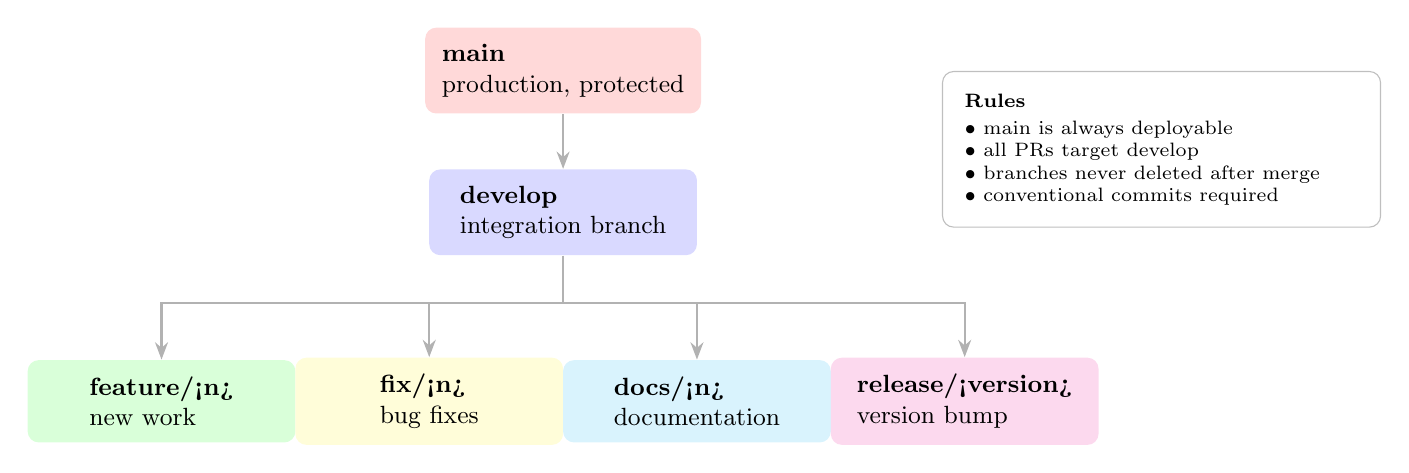
\begin{tikzpicture}[
  every node/.style={font=\small},
  box/.style={rounded corners, inner sep=6pt, align=left, minimum width=3.4cm},
  arrow/.style={-{Stealth[length=2.2mm]}, thick, gray!60},
  rulebox/.style={rounded corners, draw=gray!50, inner sep=8pt, align=left, font=\scriptsize, text width=5cm}
]

% --- Main branch (top, protected) ---
\node[box, fill=red!15] (main) at (0,0) {\textbf{main}\\production, protected};

% --- Develop branch ---
\node[box, fill=blue!15] (develop) at (0,-1.8) {\textbf{develop}\\integration branch};

% --- Branch types (fanned out below develop) ---
\node[box, fill=green!15]   (feature) at (-5.1,-4.2) {\textbf{feature/<n>}\\new work};
\node[box, fill=yellow!15]  (fix)     at (-1.7,-4.2) {\textbf{fix/<n>}\\bug fixes};
\node[box, fill=cyan!15]    (docs)    at ( 1.7,-4.2) {\textbf{docs/<n>}\\documentation};
\node[box, fill=magenta!15] (release) at ( 5.1,-4.2) {\textbf{release/<version>}\\version bump};

% --- Arrows ---
\draw[arrow] (main.south) -- (develop.north);

\draw[arrow] (develop.south) |- ++(0,-0.6) -| (feature.north);
\draw[arrow] (develop.south) |- ++(0,-0.6) -| (fix.north);
\draw[arrow] (develop.south) |- ++(0,-0.6) -| (docs.north);
\draw[arrow] (develop.south) |- ++(0,-0.6) -| (release.north);

% --- Rules box ---
\node[rulebox] (rules) at (7.6,-1) {
  \textbf{Rules}\\[2pt]
  $\bullet$ main is always deployable\\
  $\bullet$ all PRs target develop\\
  $\bullet$ branches never deleted after merge\\
  $\bullet$ conventional commits required
};

\end{tikzpicture}
\caption{Git Flow --- branch hierarchy.}
\end{figure}

\subsection*{Branch Lifecycle}

\begin{figure}[H]
\centering
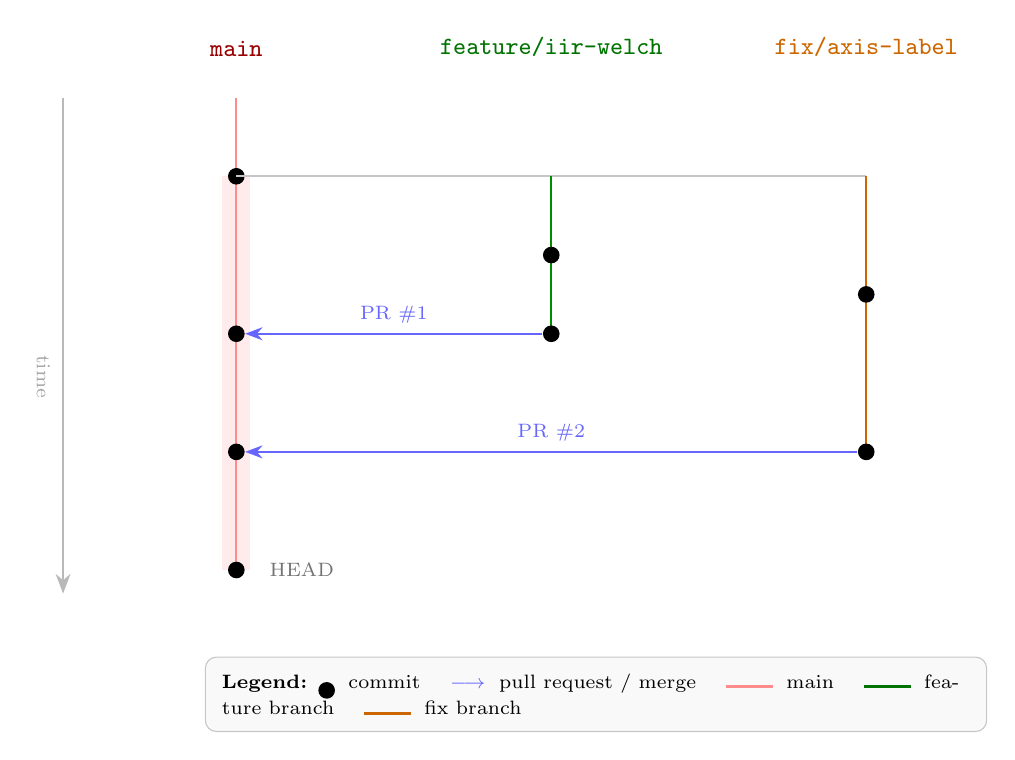
\begin{tikzpicture}[
  commit/.style={circle, fill=black, inner sep=2pt, minimum size=6pt},
  branchlabel/.style={font=\small\ttfamily\bfseries, anchor=south},
  prarrow/.style={-{Stealth[length=2.2mm]}, thick, color=blue!60},
  mainline/.style={thick, color=red!45},
  featline/.style={thick, color=green!55!black},
  fixline/.style={thick, color=orange!80!black},
]

% --- Column positions ---
\def\xtime{-2.2}
\def\xmain{0}
\def\xfeat{4}
\def\xfix{8}

% --- Column labels (top) ---
\node[branchlabel, red!60!black]        at (\xmain,0.4) {main};
\node[branchlabel, green!45!black]      at (\xfeat,0.4) {feature/iir-welch};
\node[branchlabel, orange!80!black]     at (\xfix,0.4)  {fix/axis-label};

% --- Main timeline (highlighted background band) ---
\fill[red!8] (\xmain-0.18,-1) rectangle (\xmain+0.18,-6);
\draw[mainline] (\xmain,0) -- (\xmain,-6);

% --- Main commits ---
\node[commit] (m1) at (\xmain,-1)   {}; % initial commit, both branches fork here
\node[commit] (m2) at (\xmain,-3)   {}; % PR #1 (feature) merged
\node[commit] (m3) at (\xmain,-4.5) {}; % PR #2 (fix) merged
\node[commit] (m4) at (\xmain,-6)   {}; % HEAD
\node[smalllabel, anchor=west] at (\xmain+0.3,-6) {HEAD};

% --- Fork rail: both branches are created from the same commit on main ---
\draw[gray!45, thick] (\xmain,-1) -- (\xfix,-1);

% --- feature/iir-welch branch (forks at m1, merges at m2) ---
\draw[featline] (\xfeat,-1) -- (\xfeat,-3);
\node[commit] (f1) at (\xfeat,-2) {};
\node[commit] (f2) at (\xfeat,-3) {}; % merge point, same height as m2

% --- fix/axis-label branch (forks at m1, merges at m3) ---
\draw[fixline] (\xfix,-1) -- (\xfix,-4.5);
\node[commit] (x1) at (\xfix,-2.5)  {};
\node[commit] (x2) at (\xfix,-4.5) {}; % merge point, same height as m3

% --- Merge / PR arrows back into main (plain horizontal -- no overlap) ---
\draw[prarrow] (f2) -- (m2) node[midway, above, smalllabel, color=blue!60] {PR \#1};
\draw[prarrow] (x2) -- (m3) node[midway, above, smalllabel, color=blue!60] {PR \#2};

% --- Time axis ---
\draw[-{Stealth[length=2.5mm]}, thick, gray!55] (\xtime,0) -- (\xtime,-6.3);
\node[smalllabel, gray!70, anchor=west, rotate=-90] at (\xtime-0.25,-3.15) {time};

% --- Legend ---
\node[notebox, text width=9.5cm, anchor=north west, font=\scriptsize] at (\xmain-0.4,-7.1) {
  \textbf{Legend:} \tikz[baseline=-0.5ex]{\node[commit]{};}\; commit
  \quad\textcolor{blue!60}{$\longrightarrow$}\; pull request / merge
  \quad\textcolor{red!45}{\rule{0.6cm}{1.2pt}}\; main
  \quad\textcolor{green!45!black}{\rule{0.6cm}{1.2pt}}\; feature branch
  \quad\textcolor{orange!80!black}{\rule{0.6cm}{1.2pt}}\; fix branch
};

\end{tikzpicture}
\caption{Git Flow --- parallel branches with PR merges into \texttt{main}.}
\end{figure}

%% ============================================================
\section*{Flow Sandbox 1 --- Pseudocode-Driven}

\textbf{Entry:} User provides general pseudocode.
\textbf{Exit:} Notebook merged via git flow.

\begin{figure}[H]
\centering
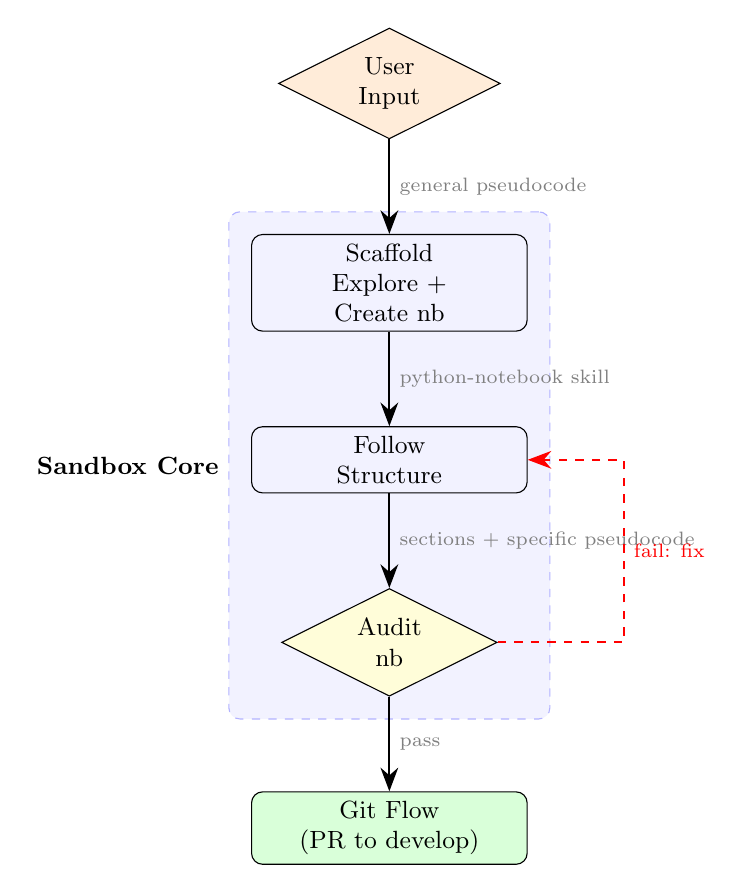
\begin{tikzpicture}[
  node distance=1.2cm,
  stage/.style={draw, rounded corners, minimum width=3.5cm, minimum height=0.8cm, align=center, font=\small},
  input/.style={draw, diamond, aspect=2, minimum width=2.5cm, align=center, font=\small, fill=orange!15},
  decision/.style={draw, diamond, aspect=2, minimum width=2.5cm, align=center, font=\small, fill=yellow!15},
  output/.style={draw, rounded corners, minimum width=3.5cm, minimum height=0.8cm, align=center, font=\small, fill=green!15},
  arrow/.style={-{Stealth[length=3mm]}, thick},
  edgelabel/.style={font=\scriptsize, color=gray}
]

% Nodes (vertical chain)
\node[input] (input) {User\\Input};
\node[stage, below=1.2cm of input] (scaffold) {Scaffold\\Explore +\\Create nb};
\node[stage, below=1.2cm of scaffold] (structure) {Follow\\Structure};
\node[decision, below=1.2cm of structure] (audit) {Audit\\nb};
\node[output, below=1.2cm of audit] (gitflow) {Git Flow\\(PR to develop)};

% Arrows
\draw[arrow] (input) -- node[right, edgelabel] {general pseudocode} (scaffold);
\draw[arrow] (scaffold) -- node[right, edgelabel] {python-notebook skill} (structure);
\draw[arrow] (structure) -- node[right, edgelabel] {sections + specific pseudocode} (audit);
\draw[arrow] (audit) -- node[right, edgelabel] {pass} (gitflow);

% Feedback loop (right side)
\draw[arrow, dashed, red] (audit.east) -- ++(1.6,0) |- node[near start, right, font=\scriptsize] {fail: fix} (structure.east);

% Background
\begin{scope}[on background layer]
  \node[draw=blue!30, dashed, rounded corners, fill=blue!5, inner sep=8pt,
        fit=(scaffold)(structure)(audit), label={[font=\small\bfseries]left:Sandbox Core}] {};
\end{scope}

\end{tikzpicture}
\caption{Flow Sandbox 1 --- pseudocode-driven pipeline.}
\end{figure}

\textbf{Steps:}
\begin{enumerate}
  \item \textbf{User Input} --- Provide general pseudocode (e.g., SDR monitoring pipeline).
  \item \textbf{Scaffold Explore + Create nb} --- Agent explores scaffold documentation, generates notebook using python-notebook skill.
  \item \textbf{Follow Structure} --- Notebook sections follow the scaffold; each section has its own specific pseudocode.
  \item \textbf{Audit nb} --- Validate: notebook format, axis conventions (N, 2, L), power calculations, missing cells.
  \item \textbf{Git Flow} --- Create feature branch, commit with conventional message, open PR to develop.
\end{enumerate}

\subsection*{Conceptual Example}

\begin{figure}[H]
\centering
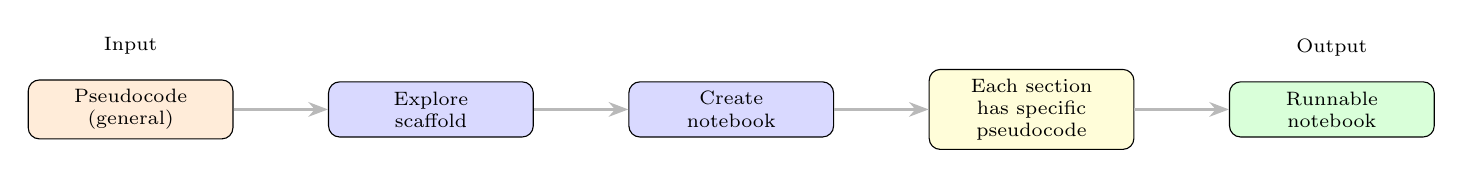
\begin{tikzpicture}[
  node distance=0.8cm and 1.2cm,
  box/.style={draw, rounded corners, minimum width=2.6cm, minimum height=0.7cm, align=center, font=\scriptsize},
  arrow/.style={-{Stealth[length=2.5mm]}, thick, gray!55},
]

% Input pseudocode
\node[box, fill=orange!15] (pseudo) {Pseudocode\\(general)};

% Processing steps
\node[box, fill=blue!15, right=of pseudo] (explore) {Explore\\scaffold};
\node[box, fill=blue!15, right=of explore] (create) {Create\\notebook};
\node[box, fill=yellow!15, right=of create] (sections) {Each section\\has specific\\pseudocode};

% Output
\node[box, fill=green!15, right=of sections] (notebook) {Runnable\\notebook};

% Arrows
\draw[arrow] (pseudo) -- (explore);
\draw[arrow] (explore) -- (create);
\draw[arrow] (create) -- (sections);
\draw[arrow] (sections) -- (notebook);

% Labels
\node[font=\scriptsize, above=0.2cm of pseudo] {Input};
\node[font=\scriptsize, above=0.2cm of notebook] {Output};

\end{tikzpicture}
\caption{Flow Sandbox 1 --- from pseudocode to runnable notebook.}
\end{figure}

%% ============================================================
\section*{Flow Sandbox 2 --- Idea-Driven}

\textbf{Entry:} Team member has a test idea (no pseudocode yet).
\textbf{Exit:} Notebook merged via git flow.

\begin{figure}[H]
\centering
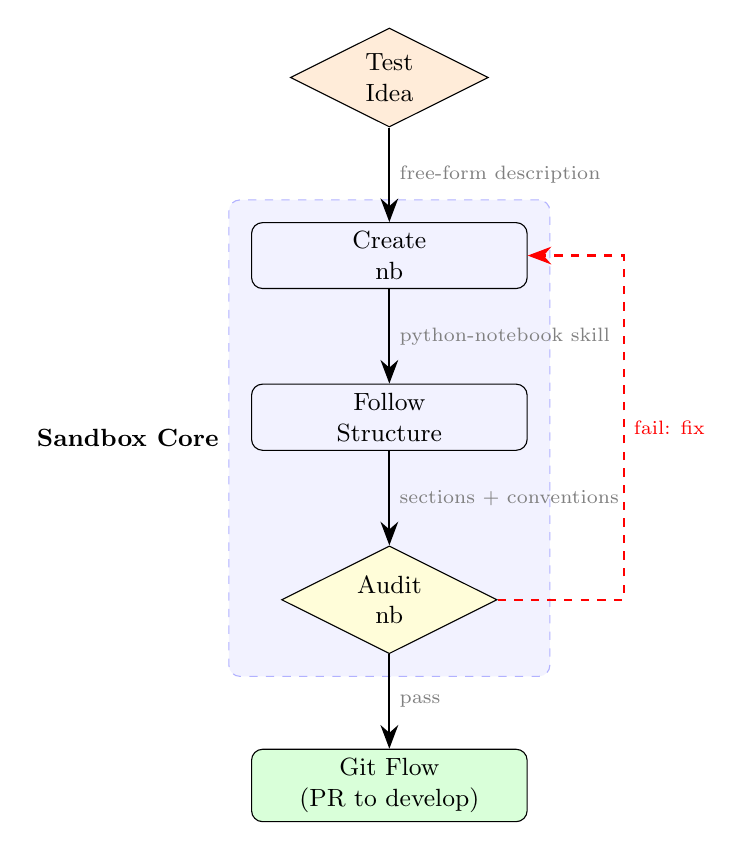
\begin{tikzpicture}[
  node distance=1.2cm,
  stage/.style={draw, rounded corners, minimum width=3.5cm, minimum height=0.8cm, align=center, font=\small},
  input/.style={draw, diamond, aspect=2, minimum width=2.5cm, align=center, font=\small, fill=orange!15},
  decision/.style={draw, diamond, aspect=2, minimum width=2.5cm, align=center, font=\small, fill=yellow!15},
  output/.style={draw, rounded corners, minimum width=3.5cm, minimum height=0.8cm, align=center, font=\small, fill=green!15},
  arrow/.style={-{Stealth[length=3mm]}, thick},
  edgelabel/.style={font=\scriptsize, color=gray}
]

% Nodes (vertical chain)
\node[input] (input) {Test\\Idea};
\node[stage, below=1.2cm of input] (nb) {Create\\nb};
\node[stage, below=1.2cm of nb] (structure) {Follow\\Structure};
\node[decision, below=1.2cm of structure] (audit) {Audit\\nb};
\node[output, below=1.2cm of audit] (gitflow) {Git Flow\\(PR to develop)};

% Arrows
\draw[arrow] (input) -- node[right, edgelabel] {free-form description} (nb);
\draw[arrow] (nb) -- node[right, edgelabel] {python-notebook skill} (structure);
\draw[arrow] (structure) -- node[right, edgelabel] {sections + conventions} (audit);
\draw[arrow] (audit) -- node[right, edgelabel] {pass} (gitflow);

% Feedback loop (right side)
\draw[arrow, dashed, red] (audit.east) -- ++(1.6,0) |- node[near start, right, font=\scriptsize] {fail: fix} (nb.east);

% Background
\begin{scope}[on background layer]
  \node[draw=blue!30, dashed, rounded corners, fill=blue!5, inner sep=8pt,
        fit=(nb)(structure)(audit), label={[font=\small\bfseries]left:Sandbox Core}] {};
\end{scope}

\end{tikzpicture}
\caption{Flow Sandbox 2 --- idea-driven pipeline.}
\end{figure}

\textbf{Steps:}
\begin{enumerate}
  \item \textbf{Test Idea} --- Team member describes what they want to test (e.g., compare Welch vs periodogram for weak signals).
  \item \textbf{Create nb} --- Agent generates notebook using python-notebook skill from the description.
  \item \textbf{Follow Structure} --- Notebook follows scaffold conventions: IQ shape (N, 2, L), axis explanations, power formulas.
  \item \textbf{Audit nb} --- Validate format, conventions, missing cells, correctness.
  \item \textbf{Git Flow} --- Branch, commit, PR to develop.
\end{enumerate}

\subsection*{Conceptual Example}

\begin{figure}[H]
\centering
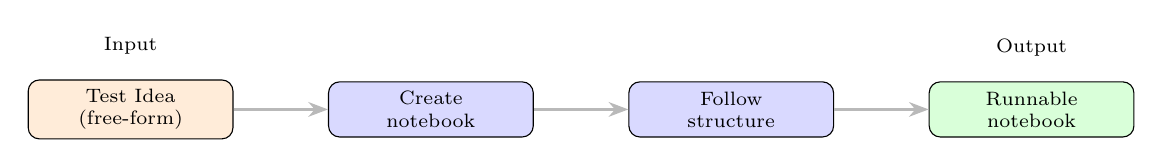
\begin{tikzpicture}[
  node distance=0.8cm and 1.2cm,
  box/.style={draw, rounded corners, minimum width=2.6cm, minimum height=0.7cm, align=center, font=\scriptsize},
  arrow/.style={-{Stealth[length=2.5mm]}, thick, gray!55},
]

% Input idea
\node[box, fill=orange!15] (idea) {Test Idea\\(free-form)};

% Processing steps
\node[box, fill=blue!15, right=of idea] (create) {Create\\notebook};
\node[box, fill=blue!15, right=of create] (structure) {Follow\\structure};

% Output
\node[box, fill=green!15, right=of structure] (notebook) {Runnable\\notebook};

% Arrows
\draw[arrow] (idea) -- (create);
\draw[arrow] (create) -- (structure);
\draw[arrow] (structure) -- (notebook);

% Labels
\node[font=\scriptsize, above=0.2cm of idea] {Input};
\node[font=\scriptsize, above=0.2cm of notebook] {Output};

\end{tikzpicture}
\caption{Flow Sandbox 2 --- from idea to runnable notebook.}
\end{figure}

%% ============================================================
\section*{What Is Missing}

The sandbox is functional but incomplete. These components need to be built:

\subsection*{1. Dockerization}

Reproducible environment for all team members.

\begin{figure}[H]
\centering
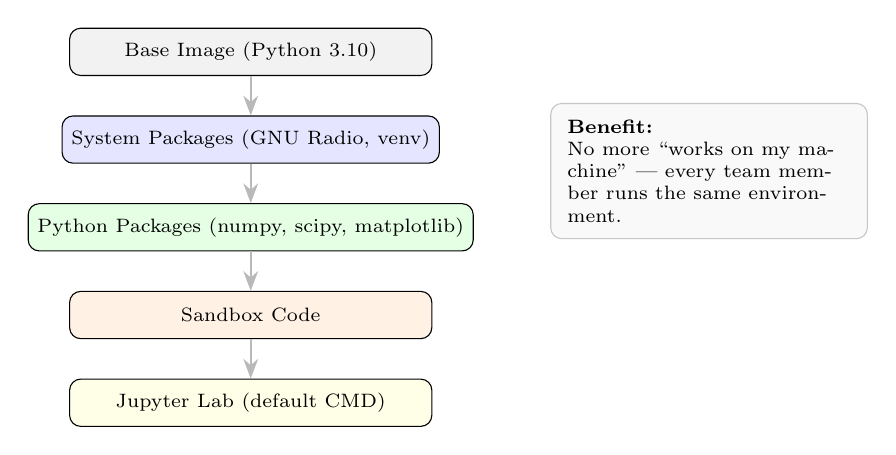
\begin{tikzpicture}[
  node distance=0.5cm,
  layer/.style={draw, rounded corners, minimum width=4.6cm, minimum height=0.6cm, align=center, font=\scriptsize},
  arrow/.style={-{Stealth[length=2.5mm]}, thick, gray!55},
]

% Docker layers
\node[layer, fill=gray!10]  (base)    {Base Image (Python 3.10)};
\node[layer, fill=blue!10]  (system)  [below=of base]   {System Packages (GNU Radio, venv)};
\node[layer, fill=green!10] (python)  [below=of system] {Python Packages (numpy, scipy, matplotlib)};
\node[layer, fill=orange!10](sandbox) [below=of python] {Sandbox Code};
\node[layer, fill=yellow!10](jupyter) [below=of sandbox]{Jupyter Lab (default CMD)};

% Arrows
\draw[arrow] (base) -- (system);
\draw[arrow] (system) -- (python);
\draw[arrow] (python) -- (sandbox);
\draw[arrow] (sandbox) -- (jupyter);

% Annotation
\node[notebox, right=1.4cm of system, yshift=-0.4cm] {
  \textbf{Benefit:}\\
  No more ``works on my machine'' --- every team member runs the same environment.
};

\end{tikzpicture}
\caption{Dockerization --- layered container structure.}
\end{figure}

\subsection*{2. Dataset Generation (Simulated)}

Synthetic IQ data for testing without hardware.

\begin{figure}[H]
\centering
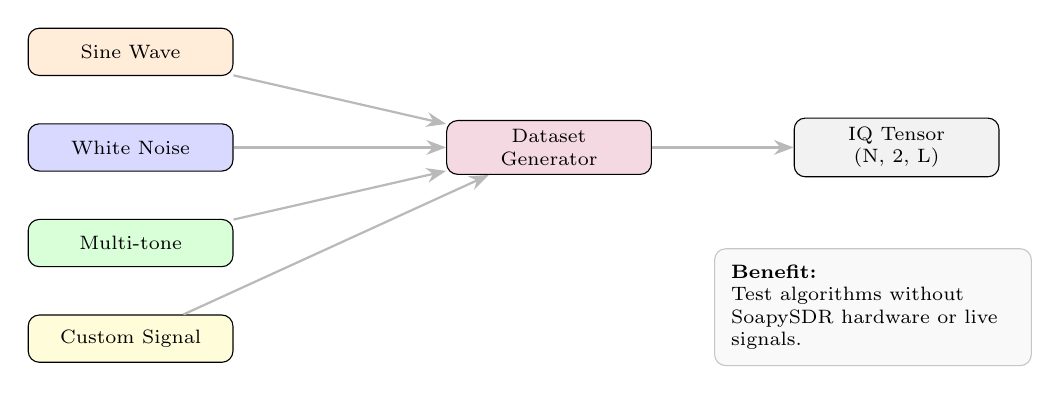
\begin{tikzpicture}[
  node distance=0.6cm and 1.8cm,
  box/.style={draw, rounded corners, minimum width=2.6cm, minimum height=0.6cm, align=center, font=\scriptsize},
  arrow/.style={-{Stealth[length=2.5mm]}, thick, gray!55},
]

% Signal types
\node[box, fill=orange!15] (sine)   {Sine Wave};
\node[box, fill=blue!15]   (noise)  [below=of sine]  {White Noise};
\node[box, fill=green!15]  (multi)  [below=of noise] {Multi-tone};
\node[box, fill=yellow!15] (custom) [below=of multi] {Custom Signal};

% Generator
\node[box, fill=purple!15, right=of noise, xshift=0.9cm] (gen) {Dataset\\Generator};

% Output
\node[box, fill=gray!10, right=1.8cm of gen] (iq) {IQ Tensor\\(N, 2, L)};

% Arrows
\draw[arrow] (sine) -- (gen);
\draw[arrow] (noise) -- (gen);
\draw[arrow] (multi) -- (gen);
\draw[arrow] (custom) -- (gen);
\draw[arrow] (gen) -- (iq);

% Annotation
\node[notebox, below=0.9cm of iq, xshift=-0.3cm] {
  \textbf{Benefit:}\\
  Test algorithms without SoapySDR hardware or live signals.
};

\end{tikzpicture}
\caption{Dataset Generation --- synthetic IQ signal types.}
\end{figure}

\subsection*{3. SoapySDR Skill}

Skill for interacting with SDR hardware via SoapySDR.

\begin{figure}[H]
\centering
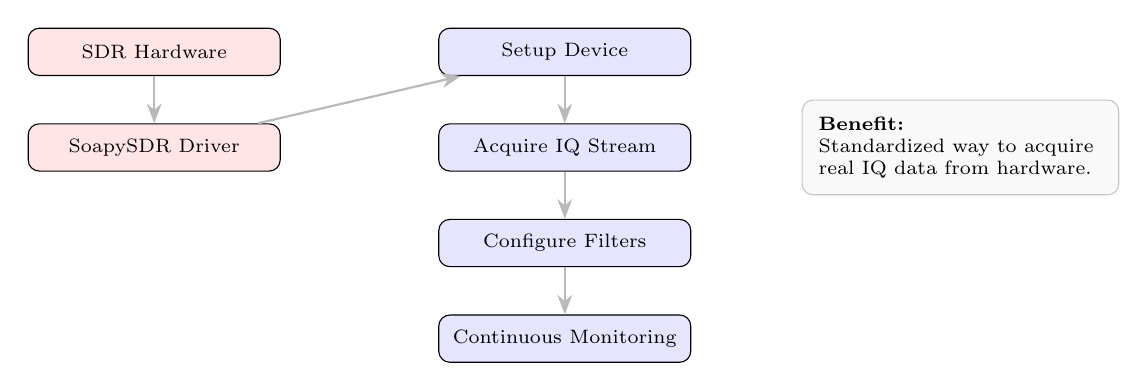
\begin{tikzpicture}[
  node distance=0.6cm and 2cm,
  box/.style={draw, rounded corners, minimum width=3.2cm, minimum height=0.6cm, align=center, font=\scriptsize},
  hw/.style={box, fill=red!10},
  sw/.style={box, fill=blue!10},
  arrow/.style={-{Stealth[length=2.5mm]}, thick, gray!55},
]

% Hardware layer
\node[hw] (sdr) {SDR Hardware};
\node[hw, below=of sdr] (driver) {SoapySDR Driver};

% Software layer
\node[sw, right=of sdr]     (setup)   {Setup Device};
\node[sw, below=0.6cm of setup]   (acquire) {Acquire IQ Stream};
\node[sw, below=0.6cm of acquire] (filter)  {Configure Filters};
\node[sw, below=0.6cm of filter]  (monitor) {Continuous Monitoring};

% Arrows
\draw[arrow] (sdr) -- (driver);
\draw[arrow] (driver) -- (setup);
\draw[arrow] (setup) -- (acquire);
\draw[arrow] (acquire) -- (filter);
\draw[arrow] (filter) -- (monitor);

% Annotation
\node[notebox, right=1.4cm of acquire] {
  \textbf{Benefit:}\\
  Standardized way to acquire real IQ data from hardware.
};

\end{tikzpicture}
\caption{SoapySDR Skill --- hardware to software interface.}
\end{figure}

\subsection*{4. Audit Skill}

Automated notebook validation.

\begin{figure}[H]
\centering
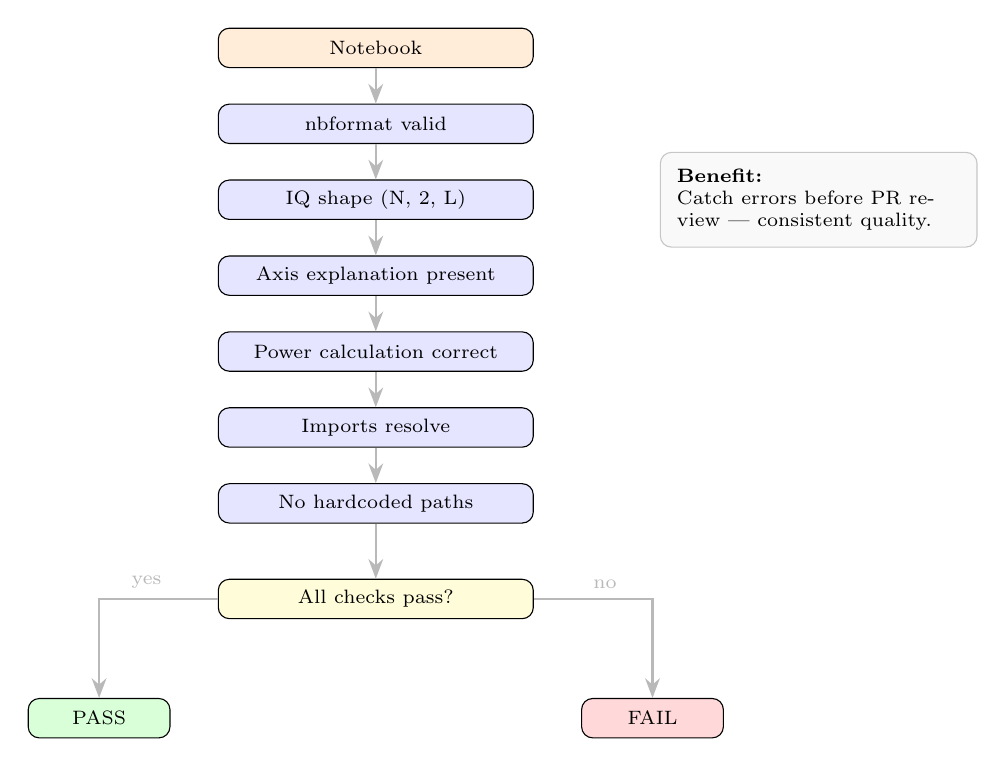
\begin{tikzpicture}[
  node distance=0.45cm,
  check/.style={draw, rounded corners, minimum width=4cm, minimum height=0.5cm, align=center, font=\scriptsize},
  input/.style={check, fill=orange!15},
  passbox/.style={check, minimum width=1.8cm, fill=green!15},
  failbox/.style={check, minimum width=1.8cm, fill=red!15},
  arrow/.style={-{Stealth[length=2.5mm]}, thick, gray!55},
]

% Input
\node[input] (notebook) {Notebook};

% Checks
\node[check, fill=blue!10, below=of notebook] (nbformat) {nbformat valid};
\node[check, fill=blue!10, below=of nbformat] (shape)    {IQ shape (N, 2, L)};
\node[check, fill=blue!10, below=of shape]    (axes)     {Axis explanation present};
\node[check, fill=blue!10, below=of axes]     (power)    {Power calculation correct};
\node[check, fill=blue!10, below=of power]    (imports)  {Imports resolve};
\node[check, fill=blue!10, below=of imports]  (paths)    {No hardcoded paths};

% Decision
\node[check, fill=yellow!15, below=0.7cm of paths] (decision) {All checks pass?};

% Outputs
\node[passbox, below left=1cm and 0.6cm of decision] (pass) {PASS};
\node[failbox, below right=1cm and 0.6cm of decision] (fail) {FAIL};

% Arrows
\draw[arrow] (notebook) -- (nbformat);
\draw[arrow] (nbformat) -- (shape);
\draw[arrow] (shape) -- (axes);
\draw[arrow] (axes) -- (power);
\draw[arrow] (power) -- (imports);
\draw[arrow] (imports) -- (paths);
\draw[arrow] (paths) -- (decision);
\draw[arrow] (decision) -| node[pos=0.3, above, font=\scriptsize] {yes} (pass);
\draw[arrow] (decision) -| node[pos=0.3, above, font=\scriptsize] {no}  (fail);

% Annotation
\node[notebox, right=1.6cm of shape] {
  \textbf{Benefit:}\\
  Catch errors before PR review --- consistent quality.
};

\end{tikzpicture}
\caption{Audit Skill --- automated validation checklist.}
\end{figure}

\subsection*{5. Harness Logic / MCP Server}

Orchestrate the full pipeline as a single command.

\begin{figure}[H]
\centering
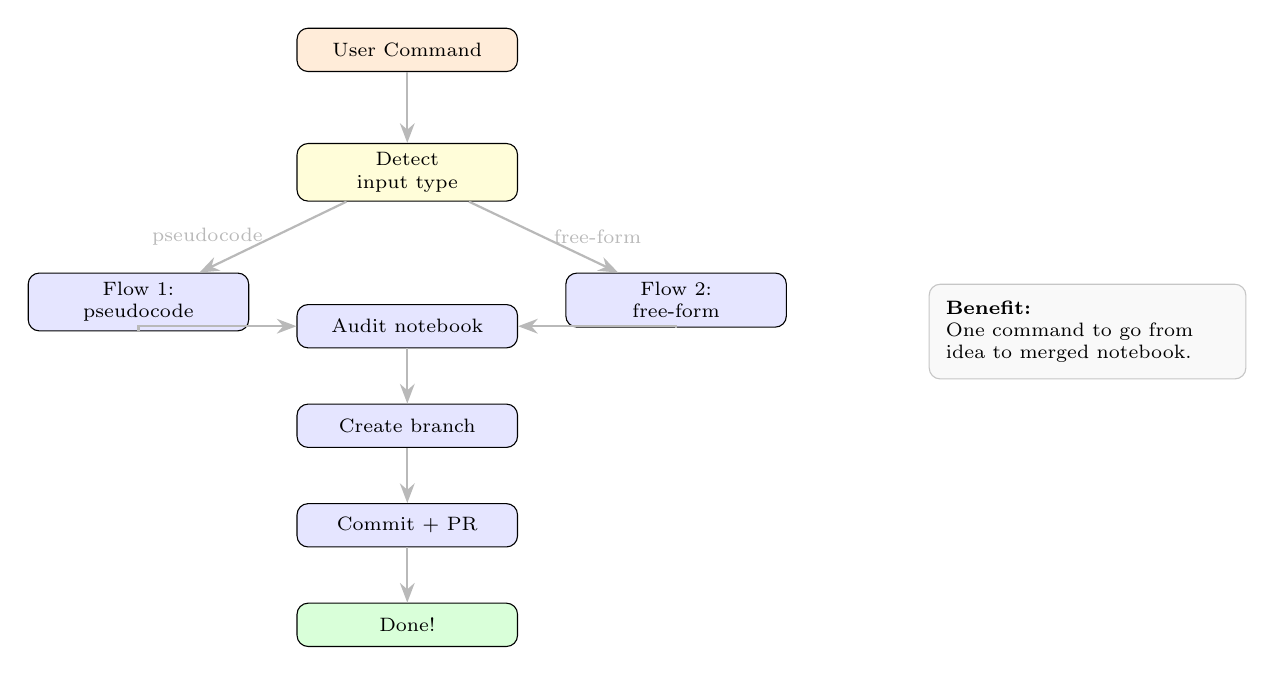
\begin{tikzpicture}[
  node distance=0.7cm,
  box/.style={draw, rounded corners, minimum width=2.8cm, minimum height=0.55cm, align=center, font=\scriptsize},
  input/.style={box, fill=orange!15},
  process/.style={box, fill=blue!10},
  output/.style={box, fill=green!15},
  arrow/.style={-{Stealth[length=2.5mm]}, thick, gray!55},
]

% Input
\node[input] (input) {User Command};

% Decision
\node[box, fill=yellow!15, below=0.9cm of input] (detect) {Detect\\input type};

% Flows
\node[process, below left=0.9cm and 0.6cm of detect]  (flow1) {Flow 1:\\pseudocode};
\node[process, below right=0.9cm and 0.6cm of detect] (flow2) {Flow 2:\\free-form};

% Shared steps
\node[process, below=1.3cm of detect] (audit)  {Audit notebook};
\node[process, below=of audit]  (branch) {Create branch};
\node[process, below=of branch] (commit) {Commit + PR};

% Output
\node[output, below=of commit] (done) {Done!};

% Arrows
\draw[arrow] (input) -- (detect);
\draw[arrow] (detect) -- node[left, font=\scriptsize] {pseudocode} (flow1);
\draw[arrow] (detect) -- node[right, font=\scriptsize] {free-form} (flow2);
\draw[arrow] (flow1) |- (audit);
\draw[arrow] (flow2) |- (audit);
\draw[arrow] (audit) -- (branch);
\draw[arrow] (branch) -- (commit);
\draw[arrow] (commit) -- (done);

% Annotation
\node[notebox, right=1.8cm of flow2, yshift=-0.4cm] {
  \textbf{Benefit:}\\
  One command to go from idea to merged notebook.
};

\end{tikzpicture}
\caption{Harness --- single-command orchestration.}
\end{figure}

%% ============================================================
\section*{Sandbox Architecture --- Full View}

\begin{figure}[H]
\centering
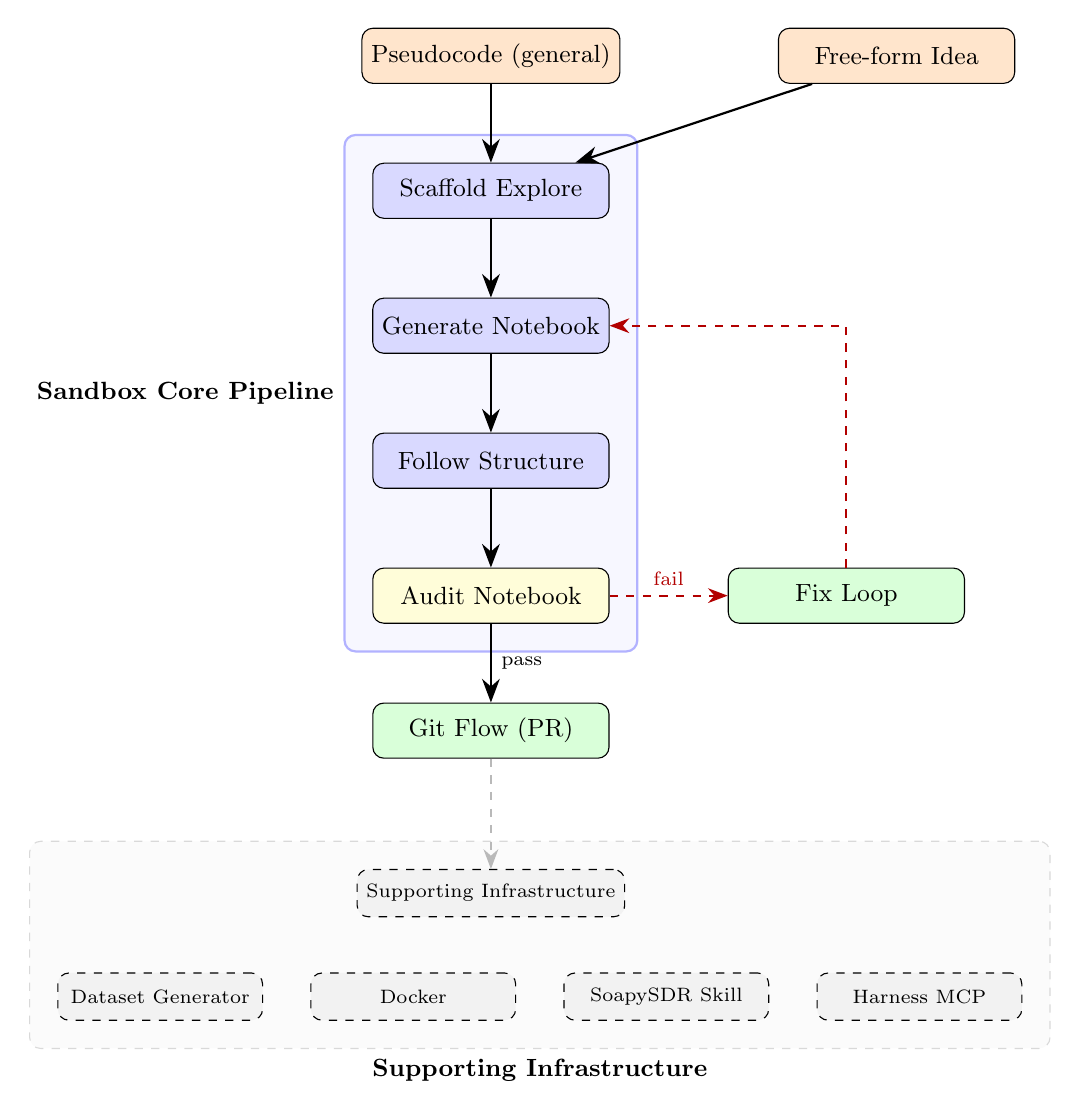
\begin{tikzpicture}[
  node distance=0.8cm,
  box/.style={draw, rounded corners, minimum width=3cm, minimum height=0.7cm, align=center, font=\small},
  input/.style={box, fill=orange!20},
  process/.style={box, fill=blue!15},
  decision/.style={box, fill=yellow!15},
  output/.style={box, fill=green!15},
  support/.style={box, minimum width=2.6cm, minimum height=0.6cm, font=\scriptsize, fill=gray!10, dashed},
  arrow/.style={-{Stealth[length=3mm]}, thick},
]

% Input layer (top)
\node[input] (pseudo) {Pseudocode (general)};
\node[input, right=2cm of pseudo] (freeform) {Free-form Idea};

% Generation layer
\node[process, below=1cm of pseudo] (scaffold) {Scaffold Explore};
\node[process, below=1cm of scaffold] (gen) {Generate Notebook};
\node[process, below=1cm of gen] (follow) {Follow Structure};

% Validation layer
\node[decision, below=1cm of follow] (audit) {Audit Notebook};
\node[output, below=1cm of audit] (gitflow) {Git Flow (PR)};

% Feedback
\node[output, right=1.5cm of audit] (fix) {Fix Loop};

% Supporting tools (bottom row, evenly spaced under a shared header)
\node[support, below=1.4cm of gitflow] (infra) {Supporting Infrastructure};
\node[support, below=0.7cm of infra, xshift=-4.2cm] (dataset) {Dataset Generator};
\node[support, right=0.6cm of dataset] (docker)  {Docker};
\node[support, right=0.6cm of docker]  (soapy)   {SoapySDR Skill};
\node[support, right=0.6cm of soapy]   (harness) {Harness MCP};

% Arrows - main flow
\draw[arrow] (pseudo) -- (scaffold);
\draw[arrow] (freeform) -- (scaffold);
\draw[arrow] (scaffold) -- (gen);
\draw[arrow] (gen) -- (follow);
\draw[arrow] (follow) -- (audit);
\draw[arrow] (audit) -- node[right, font=\scriptsize] {pass} (gitflow);
\draw[dashedarrow] (audit) -- node[above, font=\scriptsize] {fail} (fix);
\draw[dashedarrow] (fix) |- (gen);

% Arrows to infrastructure
\draw[flowarrow, dashed] (gitflow) -- (infra);

% Background
\begin{scope}[on background layer]
  \node[draw=blue!30, thick, rounded corners, fill=blue!3, inner sep=10pt,
        fit=(scaffold)(gen)(follow)(audit),
        label={[font=\small\bfseries]left:Sandbox Core Pipeline}] {};
  \node[draw=gray!30, dashed, rounded corners, fill=gray!3, inner sep=10pt,
        fit=(infra)(dataset)(docker)(soapy)(harness),
        label={[font=\small\bfseries]below:Supporting Infrastructure}] {};
\end{scope}

\end{tikzpicture}
\caption{Sandbox architecture --- core pipeline and supporting infrastructure.}
\end{figure}

%% ============================================================
\section*{Summary}

\begin{longtable}{lll}
\toprule
\textbf{Component} & \textbf{Status} & \textbf{Purpose} \\
\midrule
\endhead
pseudocode-general & Done & High-level flow description \\
pseudocode-specific & Done & Detailed algorithm design \\
python-notebook & Done & Generate notebook from description \\
project-scaffold & Done & 3-layer documentation navigation \\
git-flow & Done & Branch strategy, PR workflow \\
Dockerization & \textbf{Missing} & Reproducible team environment \\
Dataset Generation & \textbf{Missing} & Synthetic IQ data for testing \\
SoapySDR Skill & \textbf{Missing} & Hardware IQ acquisition \\
Audit Skill & \textbf{Missing} & Automated notebook validation \\
Harness / MCP & \textbf{Missing} & Orchestrate full pipeline \\
\bottomrule
\end{longtable}

\end{document}